\documentclass[tikz,border=16pt]{standalone}
\usepackage[T1]{fontenc}
\usetikzlibrary{calc}
\definecolor{espresso}{HTML}{9A5941}
\definecolor{milk}{HTML}{4B7F9B}
\definecolor{cold}{HTML}{458D79}
\definecolor{ink}{HTML}{27313A}
\begin{document}
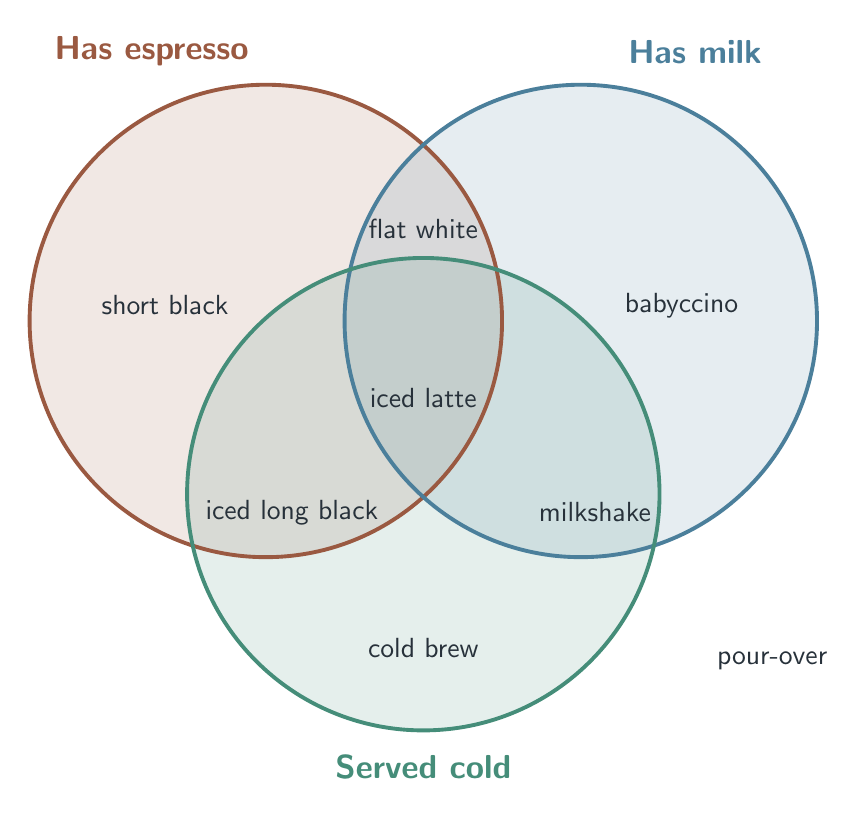
\begin{tikzpicture}[font=\sffamily, every node/.style={text=ink}]
  % Three softly tinted sets, with separately drawn boundaries.
  \fill[espresso,opacity=.14] (-2,0.8) circle (3);
  \fill[milk,opacity=.14] (2,0.8) circle (3);
  \fill[cold,opacity=.14] (0,-1.4) circle (3);
  \draw[espresso,line width=1.4pt] (-2,0.8) circle (3);
  \draw[milk,line width=1.4pt] (2,0.8) circle (3);
  \draw[cold,line width=1.4pt] (0,-1.4) circle (3);

  % Set names sit outside their circles; the colours match the outlines.
  \node[text=espresso,font=\sffamily\bfseries\large] at (-3.45,4.22) {Has espresso};
  \node[text=milk,font=\sffamily\bfseries\large] at (3.45,4.22) {Has milk};
  \node[text=cold,font=\sffamily\bfseries\large] at (0,-4.86) {Served cold};

  \node[align=center] at (-3.28,1.00) {short black};
  \node[align=center] at (3.28,1.00) {babyccino};
  \node[align=center] at (0,1.97) {flat white};
  \node[align=center] at (-1.67,-1.63) {iced long black};
  \node[align=center] at (2.18,-1.63) {milkshake};
  \node[align=center] at (0,-0.18) {iced latte};
  \node[align=center] at (0,-3.35) {cold brew};
  \node[align=center] at (4.43,-3.52) {pour-over};
\end{tikzpicture}
\end{document}
